\chapter{Tensor--Scalar Temporal Field}
The temporal configuration is represented by a scalar pace together with a rank-two relational response sector. The scalar component is typed by the internal elapsed density
\[
\boxed{
\phi
=\frac{d\tau_{\rm int}}{d\lambda}
=\frac{\mathfrak a}{\mathfrak a_\star}>0.
}
\]
For the same ordering increment \(d\lambda\), distinct admitted relational states may therefore realize distinct internal elapsed increments.

The tensorial response is written locally as
\[
\boxed{
\mathcal R^{AB}=G^{AB}+\Omega^{AB},
}
\]
where
\[
G^{AB}=G^{BA},
\qquad
\Omega^{AB}=-\Omega^{BA}.
\]
The symmetric positive sector maps the informational covector to dissipative state transport,
\[
V_I^A=-G^{AB}\partial_B\mathcal I,
\]
while the antisymmetric sector maps a local exact phase covector to reversible state transport,
\[
V_H^A=\Omega^{AB}\partial_B\mathcal H_\alpha.
\]

Formalism 01C supplies the stationary Shannon informational scalar
\[
\boxed{
\mathcal I_\pi[p]=D_{\rm KL}^{(2)}(p\|\pi).
}
\]
For admitted stationary transition dynamics this scalar contracts. In the detailed-balance sector, Formalism 01D derives the exact symmetric response
\[
\boxed{
G^{(2)}_\pi(p)
=(\ln2)D^\top\operatorname{diag}[c_{ab}\Lambda(r_a,r_b)]D,
\qquad
r_a=\frac{p_a}{\pi_a},
}
\]
and the exact flow identity
\[
\boxed{
\dot p=-G^{(2)}_\pi(p)\nabla_p\mathcal I_\pi.
}
\]
The mass-conservation direction satisfies
\[
G^{(2)}_\pi\mathbf1=0,
\]
so the corresponding metric response is taken on the active simplex tangent quotient. At uniform zero-drive equilibrium,
\[
\boxed{
G^{(2)}_u(u)=\frac{\ln2}{m}K_0,
}
\]
which ties the symmetric information-response tensor directly to the relational-mobility Laplacian used by Temporal Wave.

In the admitted Kähler factorization on a compatible active sector,
\[
g_{K,AB}=(G^{-1})_{AB},
\qquad
\Omega^{AB}=J^A{}_{C}G^{CB},
\]
where the inverse is understood on the nondegenerate tangent sector when conservation constraints are present. On an exact phase patch the evolution law is
\[
\boxed{
\frac{dx}{d\lambda}
=-\operatorname{grad}_{g_K}\mathcal I
+J\operatorname{grad}_{g_K}\mathcal H_\alpha.
}
\]
This form is the coordinate-covariant factorization of the symmetric informational-response channel and the antisymmetric local phase-response channel established in Formalism 01A.

Formalism 01B supplies the global phase completion. The edge link
\[
L_e=G_e\exp\!\left[i\kappa(\Delta H_e+\sigma_e)\right]
\]
defines a temporal connection class whose closed-cycle holonomy is
\[
\boxed{
\Phi_T(C)=\gamma_B(C)+\kappa\sum_{e\in C}\sigma_e\pmod{2\pi}.
}
\]
The exact Shannon part telescopes on a closed cycle. Berry holonomy and non-exact affinity provide the global connection data. Thus \(\mathcal H_\alpha\) is typed as a local exact-patch generator, while the U(1) connection carries global phase patching and cycle information.

The tensor--scalar temporal architecture is therefore summarized locally by
\[
\boxed{
\mathcal T
=\bigl(\phi,\mathcal R^{AB}\bigr),
\qquad
\phi=\frac{\mathfrak a}{\mathfrak a_\star},
\qquad
\mathcal R^{AB}=G^{AB}+J^A{}_{C}G^{CB},
}
\]
with a global phase-connection layer supplying the holonomy class. The scalar answers how much internal elapsed time is realized per ordering increment. The symmetric tensorial sector has a Shannon--Onsager realization in probability coordinates, while the antisymmetric/connection sector carries orientation and circulation.

The next upstream task is to extend the response decomposition to stationary nonreversible dynamics while retaining the 01C relative-information contraction and the 01B connection/current structure. Downstream realizations are tested through Temporal Wave, NOW, Bifurcation, Transport, Memory and Retrodiction.

\section{nD slices of the tensor--scalar field}
Because the full tensor--scalar state lives in a space of dimension higher than two, Figure~\ref{fig:nd-slices} provides four schematic two-dimensional slices as a readable proxy for the richer field geometry.
\begin{figure}[H]
  \centering
  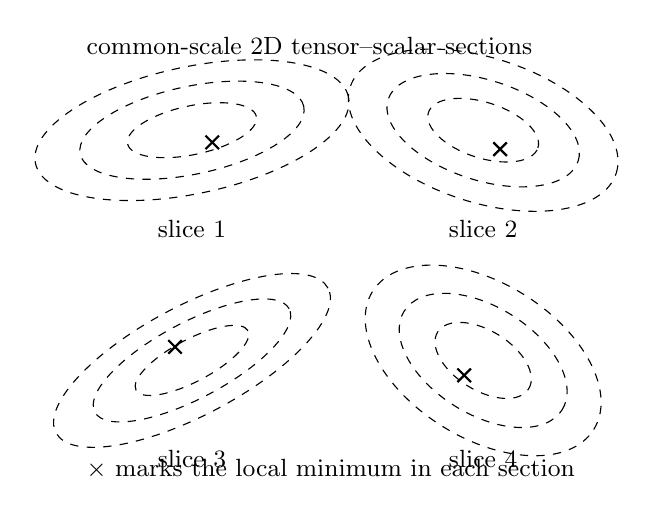
\begin{tikzpicture}[scale=0.86]
    \foreach \x/\y/\ang/\sx/\sy/\mx/\my/\lab in {
      -3.3/2.0/12/1.35/0.72/-3.0/1.82/{slice 1},
       1.0/2.0/-18/1.18/0.82/1.25/1.72/{slice 2},
      -3.3/-1.4/28/1.30/0.62/-3.55/-1.20/{slice 3},
       1.0/-1.4/-32/1.10/0.88/0.72/-1.62/{slice 4}}
    {
      \begin{scope}[shift={(\x,\y)},rotate=\ang]
        \draw[dashed] (0,0) ellipse ({1.75*\sx} and {1.30*\sy});
        \draw[dashed] (0,0) ellipse ({1.25*\sx} and {0.90*\sy});
        \draw[dashed] (0,0) ellipse ({0.72*\sx} and {0.50*\sy});
      \end{scope}
      \draw[thick] (\mx-0.10,\my-0.10) -- (\mx+0.10,\my+0.10);
      \draw[thick] (\mx-0.10,\my+0.10) -- (\mx+0.10,\my-0.10);
      \node[font=\small] at (\x,\y-1.45) {\lab};
    }
    \node[font=\small,anchor=west] at (-5.0,3.25) {common-scale 2D tensor--scalar sections};
    \node[font=\small,anchor=west] at (-5.0,-3.0) {$\times$ marks the local minimum in each section};
  \end{tikzpicture}
  \caption{Schematic four common-scale two-dimensional slices of a higher-dimensional tensor--scalar surrogate. The fixed tensor coordinates deform the local informational landscape; the cross marks the minimum in each slice.}
  \label{fig:nd-slices}
\end{figure}
